\documentclass{article}
\usepackage[utf8]{inputenc}
\usepackage{graphicx}
\usepackage[ruled, lined, linesnumbered, commentsnumbered, longend]{algorithm2e}
\usepackage{xcolor}
\usepackage{mathtools}
\usepackage{blindtext}
\usepackage{multicol}
\usepackage{sectsty}
\usepackage[]{algorithm2e}
\usepackage[english]{babel}
\usepackage[square,numbers]{natbib}
\usepackage[colorlinks, citecolor = black, urlcolor = gray, bookmarks = false, hypertexnames = true ]{hyperref} 
\bibliographystyle{abbrvnat}
\usepackage{scrextend}
\newcommand\footnoteref[1]{\protected@xdef\@thefnmark{\ref{#1}}\@footnotemark}
\usepackage{titlesec}
\titleformat*{\section}{\normalfont\filcenter}
\sectionfont{\fontsize{12}{12}\selectfont}
\subsectionfont{\fontsize{12}{12}\selectfont}
\usepackage[a4paper, total={170mm,257mm},left=20mm,right=20mm, top=20mm,]{geometry}
\title{\textbf{AI Learning Agent for the Battleship Game}}
\author{Bui Thanh Phu, Tran Hoang Long, Nguyen Minh Thi}
\date{}

\begin{document}
\maketitle

\begin{multicols}{2}
\textbf{\textit{Abstract}— This paper introduces the Battleship Game with the AI Learning Agent by the Reinforcement Learning method. Then, from that agent, let it play against other modes such as: Random, HuntAndTargetAgent and finally is Human. The first part of the thesis is an overview of the Battleship game. The second part analyses different designs, patterns and implementations of several heuristics and compares them. The third part is an overview of the Q-Learning algorithm and its parameters. The thesis also contains an outline of the formulation of the Markov Decision Process(MDP) model based on the battleship game, as well as a brief outline of existing approaches towards the Battleship game. The last part of the paper introduces and evaluates all methods and compares the results with Q-Learning Agent.}

\renewcommand*\thesection{\Alph{section}.}
\renewcommand*{\thesubsection}{\Roman{subsection}.}
\renewcommand*{\thesubsubsection}{\arabic{subsubsection}.}

\section{INTRODUCTION}
\subsection{The Battleship game}
\subsubsection{Introduction}
Battleship, also known as a Sea Battle, is a strategy type guessing game for two players. Both players have their own grid-like board and a predefined number of ships with various lengths. At the start of the game, each of them distributes all the ships across the board, concealing them from the other player. The tiles that do not contain a part of the ship are considered the ocean. There are a few rules about ships placement that need to be adhered:
\begin{enumerate}
    \item The ships can be placed either vertically or horizontally, however not diagonally.
    \item The ships can not overlap. There is nothing in the rules to say they cannot touch. (In fact, some players consider this a strategy to confuse an opponent by obfuscating the true layout of ships. If there are five hit in a row, a naive player might consider this to be the successful destruction of an aircraft carrier of length 5, but actually it could be the sinking of a battleship of length 4, and part of a cruiser of length 3).
    \item The ships can not move during the game.
\end{enumerate}
After each player being satisfied with their layout, the game starts. The players take their turns, guessing a single tile in each round. The other player is obligated to inform the guessing player, whether the chosen tile contains a part of the ship or the ocean. If all of a player's ships have been sunk, the game is over, and their opponent wins. If both players lost all their ships in a single round, the game results in a draw.
\subsubsection{Board}
In the battleship game, the board is a two-dimensional matrix of tiles. The original game is played on the 10 × 10 board with five ships located on the board. 
\begin{center}
\begin{tabular}{|c | c|} 
 \hline
 \textbf{Type} & \textbf{Size}\\ [0.5ex] 
 \hline
 Carrier & 5 \\ 
 \hline
 Battleship & 4\\
 \hline
 Submarine & 3\\
 \hline
 Cruiser & 3\\
 \hline
 Destroyer & 2\\
 \hline
 \hline 
\end{tabular}
\\[1.5ex]Table 1: Size of ship in Battleship
\end{center}
Since the players can not move their ships (thus they can not influence their enemy's selection), we can reduce the game from two players into trying to minimize the number of moves needed to uncover all the ships of one player. In that case, we can set the end of the game to all ships being uncovered or every tile being opened.
To represent the battleship board, we use three types of tiles:
\begin{itemize}
  \item \textit{Ocean} - A tile that represents the ocean; hitting this type of tile results in a miss. Illustrated by space.
  \item \textit{Ship} - A tile that represents a part of the ship is illustrated by a dot.
\end{itemize}
\subsubsection{Actions}
If we play on the board with no tiles opened yet, obviously, there are 100 moves that can be performed, each tile representing one move. However, before actually making a move, we can observe two types of outcomes from it. Either we miss or hit the ship. That is the reason the number of actions is twice the moves available. 
\begin{center}
\textit{moves * 2 = 200 }
\end{center}
Therefore, we have 200 possible actions to perform. With each move being made, the number of actions reduces by two.
Legal move is we fire torpedo into unknown tile and has never fired before. More, it is also illegal to fire at a location off the map
\subsubsection{States}
There is a finite number of states the board can get into. Considering we do not know anything about the board unless we provide a move, at the very beginning, every layout of ships has the same probability. As the game goes on and actions are being taken, some become impossible or less probable. We have two state of each actions can happen.
\begin{itemize}
  \item \textit{Hit} - A tile that represents a part of the ship was hit by the torpedo and illustrated by X-mark.
  \item \textit{Ship} - A tile that represents the torpedo was missed and illustrated by O-mark.
\end{itemize}
\subsubsection{Reward}
Because the Battleship Game haven't the score. The game just end when all ships of either player are sunk. And that, we have the winner and the loser. But in this project, we use the Q-Learning so that we must have the reward to be able to set up the algorithm.
 \begin{center}
\begin{tabular}{|c | c|} 
 \hline
 \textbf{Type} & \textbf{Score}\\ [0.5ex] 
 \hline
 Carrier & 100 \\ 
 \hline
 Battleship & 80\\
 \hline
 Submarine & 60\\
 \hline
 Cruiser & 60\\
 \hline
 Destroyer & 40\\
 \hline
 \hline 
\end{tabular}
\\[1.5ex]Table 2: Score of ship in Battleship
\end{center}
And we also add the value for each move is minus 1 point. We have the function to calculate score:
\begin{center}
\textit{score = 340 (total score of ship) - n (number of move-action)}
\end{center}
\subsubsection{Heuristics and solving approaches}
We will solve the problem of reducing the moves needed to uncover
the board entirely with many approaches. The best way would be to
set some basic number of moves with a straightforward algorithm and improve.

\begin{enumerate}
	\item \textit{NoOp Agent} - This Agent takes no action and randomly places its ships.  This Agent is used as an opponent when testing another Agent individually.
    \item \textit{Random Agent} – The first algorithm will be a player deciding randomly. Making moves without any heuristic is the starting point of every other algorithm we will be using. Therefore, we can observe the improvement of other algorithms compared to this one.
    \item \textit{HuntAndTarget Agent} - The Hunt and Target agent will randomly search the board. After hitting an enemy ship, the Hunt and Target agent will attack surrounding squares until the ship is sunk.    
    \item \textit{Q-Learning Agent} - A Q-Learning agent is a value-based reinforcement learning agent that trains a critic to estimate the return or future rewards. For a given observation, the agent selects and outputs the action for which the estimated return is greatest. In the game, Q-Learning agent will hit the position likely where the ship might be located.
    \end{enumerate}
\section{IMPLEMENTATION}
\subsection{NoOp Agent}
	This is the Agent takes no action and randomly places its ships. The Agent is use as an opponent for testing.
\subsection{Random Agent}
The first possible strategy for building a computer opponent is to make shots totally at random. As expected, the results of firing random volleys produces very poor results. Games take a long time to complete, as the majority of squares have to be hit in order to ensure that all the ships are sunk.

Mathematically, the chances of playing a perfect game with random firing are easy to calculate and are:
\begin{center}
$\dfrac{355,687,428,096,000}{2,365,369,369,446,553,061,560,941,772,800,000}$

(This equates to, on average, once in every 6,650,134,872,937,201,800 games!)
\end{center}
I ran 100 million simulations of random games, and the smallest number of moves I encountered was 44 shots.

Below is the graph showing the distribution of the number of random shots required to finish each of the 100 million simulations. The x-axis shows the number of shots, and and the y-axis shows the number of games that were completed in that number of shots.

\begin{center}
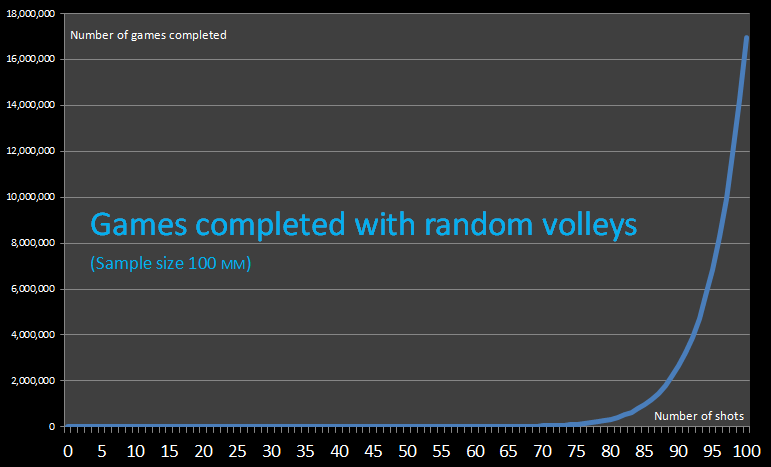
\includegraphics[scale=.35]{random}
\textit{Figure 1. The distribution of the number of random shots required to finish}
\end{center}

(It should be no surprise that number of games that required all 100 shots to be fired is 17 million. After all, there is a 17/100 chance that the last square visited will contain a ship).

Below is a graph of the cumulative probability of completing the game with n-random volleys. 96 shots are required to complete approx 50 percent of the games, and 99 percent of the games will take more than 78 shots.
\begin{center}
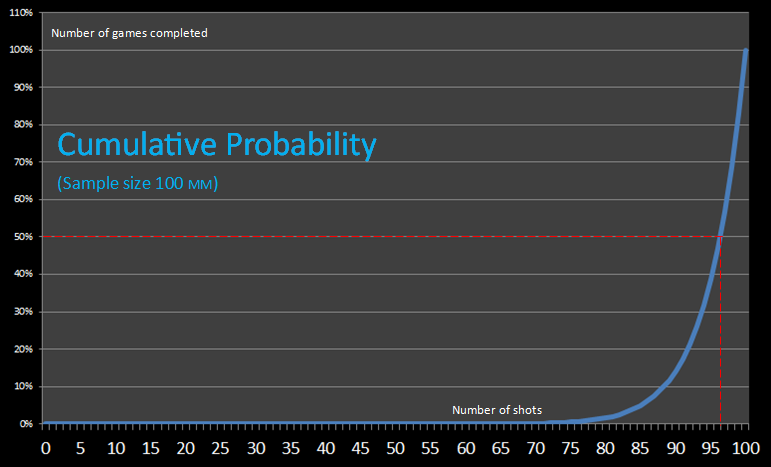
\includegraphics[scale=.35]{cumulative}
\textit{Figure 2. Cumulative Probability}
\end{center}

\subsection{Hunt And Target Agent}
It's fairly easy to greatly improve results. Initially, shots can be fired at random, but once part of a ship has been \textbf{hit}, it's possible to search up, down, left and right looking for more of the same ship.
	
A simple implementation of this refined strategy is to create a stack of potential targets. Initially, the computer is in \textbf{Hunt} mode, firing at random. Once a ship has been 'winged' then the computer switches to \textbf{Target} mode. After a \textbf{hit}, the four surrounding grid squares are added to a stack of 'potential' targets (or less than four if the cell was on an edge/corner).

Cells are only added if they have not already been visited (there is no point in re-visiting a cell if we already know that it is a \textbf{Hit} or \textbf{Miss}).

Once in \textbf{Target} mode the computer pops off the next potential target off the stack, fires a salvo at this location, acts on this (either adding more potential targets to the stack, or popping the next target location off the stack), until either all ships have been sunk, or there are no more potential targets on the stack, at which point it returns to \textbf{Hunt} mode and starts firing at random again looking for another ship.

Even though far from elegant, this algorithm produces signifincantly better results than random firing. It is, however, a long way from efficient as it has no concept of what constitutes a ship, and blindly needs to walk around all surrounding edges of every \textbf{hit} pixel (with the exception of the last hit one), making sure there are no more ships touching.

The result: Below is a graph of the results using this basic algorithm on 100 million randomly generated grids.
\begin{center}
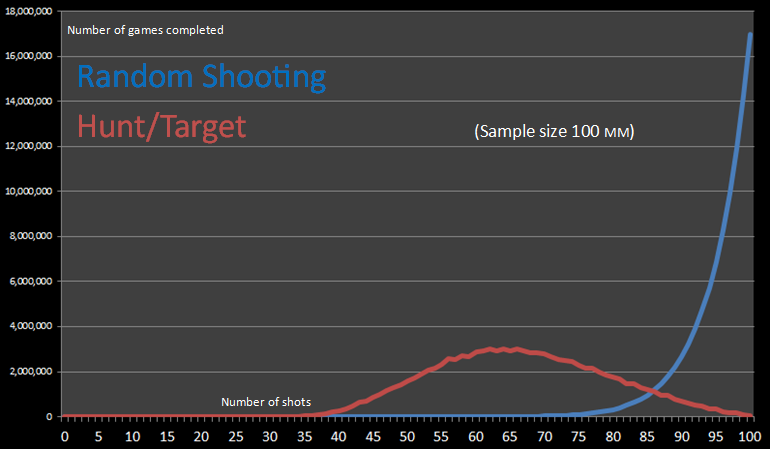
\includegraphics[scale=.35]{b1}
\textit{Figure 3. Compare between Random Agent \& Hunt and Target Agent}
\end{center}
The red line depicts the results of this algorithm and the blue line, for reference, shows the results of pure random guessing. There is an obvious improvement.
\subsection{Q-Learning Agent}
To implement an AI game agent for the game of Battleship, we are approaching the game fundamentally as an optimization problem. The task then becomes searching the state space to find the optimal policy for selecting actions, i.e. coordinates of the square to strike.

At a high level, our agent employs a reinforcement learning technique for Markov Decision Process. This approach reflects the nature of the game of Battleship, where the location of the ships are hidden from the player. With each action (square selected to strike), there is an unknown probability of transitioning to each possible successor state (either a \textbf{miss} or a \textbf{hit}), and the corresponding rewards are therefore unknown as well. But from studying the layout of the game board, it is possible for a learning agent to learn, over repeated iterations, the probability that a specific square contains a ship. 

Specifically, our algorithm is based on the Q-Learning algorithm to find the optimal policy. Each time we select a square on the game board to strike (action a), the algorithm performs value iteration to update the expected utility of selecting that square based on the result \textbf{(V(s’))}. Through this process, we eventually converge to the true expected utility and obtain the action that yields the highest expected value at each state. 
\begin{center}
$Q(s,a)=(1-\eta)Q(s,a)+\eta(r+\gamma V(s'))$

For the step size  , we scale it based on the inverse of the square of the number of iterations to gradually reduce the step size as we converge on the optimal policy, that is: 
\end{center}

\begin{footnotesize}
\begin{verbatim}
 	def getStepSize(self):
      return 1.0 / math.sqrt(self.numIters)

\end{verbatim}
\end{footnotesize}

To ensure that we are learning the optimal policy while the state space is properly explored, our agent uses the epsilon-greedy algorithm to produce the actual action. Currently, we assign epsilon to 0.1. Therefore we will generally choose the action based on policy, but for 10 percent of the time will take a random action that takes us into a new state not yet covered by the existing policy.

\begin{footnotesize}
\begin{verbatim}
 def getAction(self, state):
   self.numIters += 1
   if random.random() < self.epsilon:
     return random.choice(self.actions(state))
   else:
     return max((self.getQ(state, action), action)
      for action in self.actions(state))[1]

\end{verbatim}
\end{footnotesize}

A learning algorithm relies on the proper assignment of rewards to derive the expected utility of a policy. We use a simple scoring mechanism that is based on weighted portion of ships sunk discounted by the total number of moves executed:

{\footnotesize $Score=(\displaystyle\sum_{ships} \dfrac{Squares Hit}{Total Squares Occupied}(The Value Of Ship's)-NumberMovesTaken)$}

Each ship is assigned a value based on its size. A ship of length 5 is assigned a value of 100, a ship of length 4 has value 80, a ship of length 3 has value 60, and so forth. In essence, the algorithm can use this system to learn to sink as many ships in as few moves as possible.

A major challenge for our agent is exploring the large state-space, which increases exponentially with the game board size. Currently, our algorithm does not employ any pruning techniques to reduce the state space to be searched. Going forward, we expect to incorporate pruning to our algorithm to search the state space more quickly and efficiently.
\section{BASELINES AND ORACLES}
We are using several non-learning approaches as baselines and oracles to compare with our learning-based AI agent:
\begin{itemize}

\item	Baseline 1: A random algorithm can simply select squares at random to strike each turn. It is simple but not very interesting. We can use this to represent the absolute lower bound on effectiveness.
\item	Baseline 2: A hunt-and-target algorithm is a simple implementation that improves on the random algorithm. At first, it also selects squares at random to strike. But after a strike results in a hit, it will target the squares adjacent to the hit square during subsequent turns. 
\item 	Oracle: In general, a human can play the game of Battleship reasonably well. Most humans employ a strategy similar to the hunt-and-target approach but will subconsciously incorporate addition intuition to determine the likelihood that a square contains a ship. For example, an unexplored square that is mostly surrounded by missed strikes is not very likely to contain a ship, since a ship would likely have occupied several of the adjacent squares that have already been exposed. As such, a human would likely prioritize other squares as the target.


\end{itemize}
It is also useful to note that the theoretical upper bound to effectiveness would be 100 percent hit rate, i.e. all strikes result in a hit and the game is completed in the minimum possible number of turns. 
\section{RESULT}

\begin{center}
\begin{tabular}{|c | c| c|} 
 \hline
 \textbf{Agent} & \textbf{Average
  Moves}& \textbf{Average Score}\\ [0.5ex] 
 \hline
Random & 95 & 244.59 \\ \hline
Hunt and Target & 64 & 275.65 \\ \hline
Human & 56 & 284.00 \\ \hline
Q-Learning & 50.89 & 289.11 \\ \hline
 \hline 
\end{tabular}
\\[1.5ex]Table 3: Classic Battleship Results
\end{center}
The Random agent requires the most moves to complete the game, and receives the lowest score.  The Random agent’s poor performance can be attributed to its complete lack of any game-specific knowledge.  The Random agent will always pick a new board square to attack, even if the Random agent scored a hit on a previous attack.

The Hunt and Target agent performs much better than the Random agent, requiring about one third fewer moves to complete the game.  The Hunt and Target agent also selects its targets at random, but the Hunt and Target agent includes the game-specific knowledge that ships are oriented in straight lines on the game board, and the object of the game is to sink the opponent’s ships.  Using this knowledge, the Hunt and Target agent will attack squares surrounding a square that was a hit previously.  The Hunt and Target agent greedily attempts to sink ships it knows about, and otherwise randomly explores the game board.

A Human agent performs the best of all agents tested.  The Human agent uses 12.5 percent fewer moves to complete the game than the Hunt and Target agent.  The Human agent acts similarly to the Hunt and Target agent when attempting to sink a known ship.  However, when the Human is searching for an unknown ship, the Human is capable of visually scanning unexplored game squares and selecting the minimum amount of shots required to explore regions of the game board.  The Human knows the amount and length ships on the game board, so the Human can improve on randomly searching unexplored spaces.

The Q-Learning agent performs in between the Random and Hunt and Target agents.  The Q Learning agent is a preliminary implementation of the Q Learning algorithm with a simple identity feature extraction algorithm that memorizes states and actions.  The feature extraction algorithm does not generalize to never-before-seen states and actions at all, and does not include any game-specific features to guide the Q Learning agent.  However, the Q Learning agent is learning during each game, so in some games when a state has been seen before, the learning agent is capable of performance near the level of the Hunt and Target agent.  In most games, the severely limited feature extraction of the Q Learning agent limits performance to near the Random agent.

\end{multicols}

\end{document}

